\section{Comparison between methods}
As last step for this report we will blend together all the results achieved by the four different methods illustrated by, first, comparing the three iterative methods on time metrics and, then, by comparing all of them based on errors and residuals. Keep in mind that the results shown here and in all the tables before were achieved with starting point $x_0=0$, since we have empirically seen it to be the best choice.

\subsection{Comparison on time metrics}
We will start by considering only three of the methods seen until now (L-BFGS, CG and SMD) since thin QR is not iterative. \autoref{tab:time_comparison} shows the execution times and number of iterations achieved by the best configuration of these three methods:
\begin{itemize}
    \item For the L-BFGS method the best results were retrieved from \autoref{tab:lbfgs_results} where $l=20$.
    \item Conjugate gradient had no hyper-parameters, so the results are those seen from \autoref{tab:cg_results}.
    \item For standard momentum descent the results are those from \autoref{tab:smd_results}, following the grid search for the best values of $\beta$.
\end{itemize}

\begin{table}[H]
\centering
\begin{tabular}{c|c|c|c|c|c|c} \hline \hline
    \multirow{2}{*}{$\lambda$} & \multicolumn{2}{c|}{L-BFGS} & \multicolumn{2}{c|}{CG} & \multicolumn{2}{c}{SMD} \\ \cline{2-7}
    & time & steps & time & steps & time & steps \\ \hline \hline
    
    \rowcolor{gray!30} $10^4$ & $3.0\times10^{-3}$ & $4$ & $5.5\times 10^{-4}$ & $4$ & $9.5 \times 10^{-4}$ & 19 \\
    
    $10^2$ & $3.5\times10^{-3}$ & $10$ & $1.2\times 10^{-3}$ & $10$ & $4.1 \times 10^{-3}$ & 106 \\
    
    \rowcolor{gray!30} $1$ & $3.8\times10^{-3}$ & $13$ & $1.8\times 10^{-3}$ & $18$ & $4.9 \times 10^{-2}$ & $1350$ \\
    
    $10^{-2}$ & $3.9\times10^{-3}$ & $13$ & $1.9\times 10^{-3}$ & 17 & $3.8 \times 10^{-2}$ & $1075$ \\
    
    \rowcolor{gray!30} $10^{-4}$ & $4.0\times10^{-3}$ & $13$ & $2.0\times 10^{-3}$ & $18$ & $4.1 \times 10^{-2}$ & $1148$ \\
    \hline \hline
\end{tabular}
\caption{Comparison on execution time (in seconds) and number of iterations between the three iterative methods.}
\label{tab:time_comparison}
\end{table}

\noindent As we can see from \autoref{tab:time_comparison} L-BFGS and conjugate gradient methods performs in a similar way, instead SMD has an higher number of iterations and execution time as $\lambda$ starts to get smaller and smaller, this is expected since standard momentum descent is just a poorer version of conjugate gradient.
\vspace{3mm}

\noindent Between L-BFGS and conjugate gradient, the former has a low number of iteration but double the execution time, so, at the end, the best iterative algorithm, in our case, would be conjugate gradient.

\subsection{Comparison on metrics}
Let us now talk about the comparison on errors and residuals, this time including the results achieved by the thin QR factorization. The results are shown in \autoref{tab:errors_comparison}.
\begin{table}[H]
\centering
\begin{tabular}{c|c|c|c|c}
    \hline \hline
    \multirow{2}{*}{$\lambda$} & \multicolumn{2}{c|}{L-BFGS} & \multicolumn{2}{c}{Thin QR} \\ \cline{2-5}
    & error & residual & error & residual \\ \hline \hline
    
    \rowcolor{gray!30} $10^4$ & $1.40 \times 10^{-14}$ &$9.99 \times 10^{-1}$& $7.38 \times 10^{-14}$ & $9.99 \times 10^{-1}$  \\
    
    $10^2$ & $5.62 \times 10^{-15}$ & $9.37 \times 10^{-1}$ & $1.56\times 10^{-14}$ & $9.11 \times 10^{-1}$ \\
    
    \rowcolor{gray!30} $1$ & $1.73 \times 10^{-14}$ &$5.89 \times 10^{-2}$ & $2.03 \times 10^{-14}$ & $5.34 \times 10^{-2}$ \\
    
    $10^{-2}$ & $2.72 \times 10^{-14}$ & $5.02 \times 10^{-4}$ & $9.01 \times 10^{-14}$ & $5.44 \times 10^{-4}$ \\
    
    \rowcolor{gray!30} $10^{-4}$& $4.07 \times 10^{-14}$& $6.08 \times 10^{-6}$ & $8.17 \times 10^{-14}$ & $5.40 \times 10^{-6}$\\
    \hline
    
    \end{tabular} \\
    \begin{tabular}{c|c|c|c|c}
    \hline
    \multirow{2}{*}{$\lambda$} & \multicolumn{2}{c|}{CG} & \multicolumn{2}{c}{SMD} \\ \cline{2-5}
    & error & residual & error & residual \\ \hline \hline
    
    \rowcolor{gray!30} $10^4$ & $2.76 \times 10^{-14}$ & $ 9.99 \times 10^{-1}$& $3.49 \times 10^{-14}$ & $9.99 \times 10^{-1}$  \\
    
    $10^2$ & $ 1.47 \times 10^{-14}$ & $ 9.33 \times 10^{-1}$ & $8.67\times 10^{-14}$ & $9.39 \times 10^{-1}$ \\
    
    \rowcolor{gray!30} $1$ & $2.03\times 10^{-14}$ & $ 5.60 \times 10^{-2}$ & $3.51 \times 10^{-14}$ & $5.61 \times 10^{-2}$ \\
    
    $10^{-2}$ & $2.75 \times 10^{-14} $ & $5.54 \times 10^{-4}$ & $5.77 \times 10^{-14}$ & $5.07 \times 10^{-4}$ \\
    
    \rowcolor{gray!30} $10^{-4}$& $2.79 \times 10^{-14}$ & $5.22 \times 10^{-6}$ & $6.42 \times 10^{-14}$ & $5.42 \times 10^{-6}$\\
    \hline \hline
    
    \end{tabular}
\caption{Comparison on relative errors and residuals.}
\label{tab:errors_comparison}
\end{table}

\noindent By analyzing the errors and residuals obtained by the algorithms, we notice that they are pretty similar, and this is maybe due to the fact that our function is strongly convex, therefore, it was quite easy to find the unique global minimum and, as a consequence, we had the nice possibility to use the exact line search for those algorithm that required a line search. As we can see in \autoref{tab:errors_comparison}, in terms of relative errors, L-BFGS performs better with respect to the others, but not significantly noticing that the order of magnitude is the same of the other algorithms.
\vspace{3mm}

\noindent Another aspect to consider is that the performances of SMD and L-BFGS depend on their hyper-parameters. We are referring to the memory size $l$ for L-BFGS and to the step size $\eta$ and the momentum $\beta$ for SMD. The first hyper-parameter of the latter is useful only for the fixed step length version, that often requires a grid search before being chosen, as well as for the momentum. To clarify, the choice of a too low memory size of L-BFGS could slow down the convergence rate, but eventually the algorithm finds a solution, instead this does not happen if the learning rate is chosen wrongly, since it could cause the SMD to diverge. Rather, thin QR and conjugate gradient are ready-to-use algorithms that do not require hyper-parameters tuning, so they are easier to set up.

\subsection{Comparison on space}
Now, we can analyze these algorithms in terms of space complexity. Starting with thin QR, we notice that is the one using more memory because it stores the upper triangular matrix $R_1$ and the vector resulting from the product $Q_1 \hat{y}$, because we do not explicitly compute $Q_1$.
\vspace{3mm}

\noindent Then, we have conjugate gradient and standard momentum descent that are the lightest, in fact they only need few arrays: both require one for the solution, and one for the residual $r_k$ whereas CG needs one more for $p_k$ and SMD needs another one for the $v$ array in order to update the solution. In the end we have L-BFGS, whose space complexity is dominated by the two matrices $S,Y \in \mathbb{R}^{n\times l}$, where $n$ is the size of the solution and $l$ is the memory size, plus the same space required by the last two aforementioned algorithms. Let us say that L-BFGS uses less memory than thin QR when $l < \frac{n}{2}$, which always holds for our case since $n=1477$ and $l \in [3, 20]$.

\subsection{Comparison on scalability}
As final comparison we will compare the scalability of each method in a similar fashion to what we have done in \ref{subsec:qr_linearity}. We generated $20$ matrices and we run each every method five times on them, then we averaged the results in order to compare the methods' behavior as the size of the problem increases. As first test we fixed the number of columns to $200$ and we let the number of rows grow by $250$ at every new generated matrix, starting from $1000$. Afterwards, for the second test, we performed the same task of the first one but, this time, we also increased the number of columns by $50$ at each step to see how the methods scale when both sizes increase.
\begin{figure}[H]
    \centering
    \subfloat[Scalability by varying the number of rows \label{subfig:scalability_rows}]{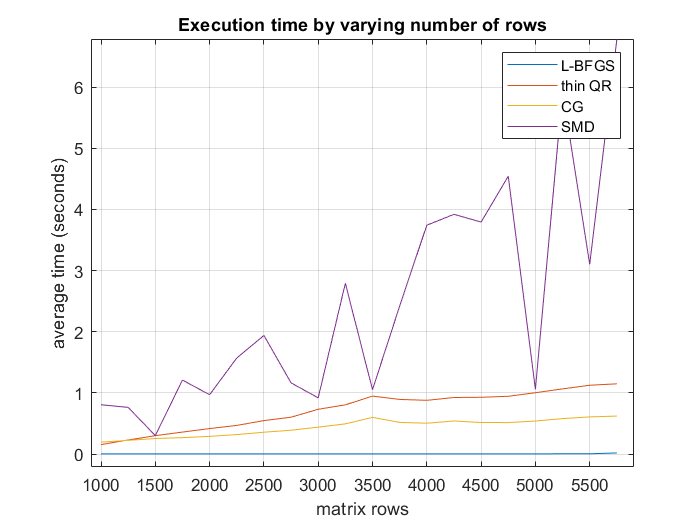
\includegraphics[width=0.5\linewidth]{images/comparisons/comparison_scalabiltiy_rows.png}}
    \subfloat[Scalabilty by varying both sizes \label{subfig:scalability}]{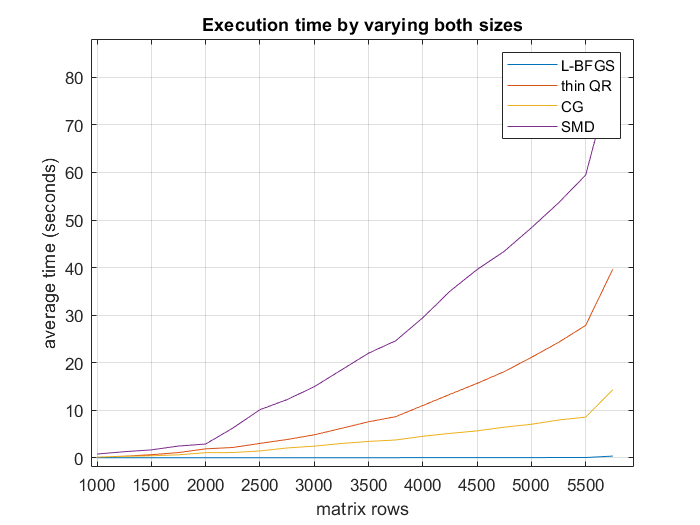
\includegraphics[width=0.5\linewidth]{images/comparisons/comparison_scalability.png}}
    \caption{Scalability comparison between the four methods, first by only varying the number of rows and then by varying both sizes.}
    \label{fig:comparison_scalability}
\end{figure}

\noindent As we can see from \autoref{fig:comparison_scalability} standard momentum descent performs worse than the other three methods since we could not do an exhaustive grid search to look for the best value of $\beta$ for each configuration. Other than that, from both figures we can notice that L-BFGS (with $l=20$) is the uncontested winner since it suffers a little from the increase in size of the matrix. Moreover, by looking at \autoref{subfig:scalability} we can see that thin QR is the one suffering the most by the increase in columns, as expected from the theory, meanwhile the others maintain, more or less, the same behavior, except for SMD which seems more stable than what we can see in \autoref{subfig:scalability_rows} at the cost of an even worse scalability.
